\documentclass[12pt]{article}

\usepackage[parfill]{parskip}
\usepackage{fancyhdr}
\usepackage[fleqn]{amsmath}
\usepackage{amssymb}
\usepackage{hyperref}
\usepackage{enumitem}
\usepackage{tikz}

\pagestyle{fancy}
\fancyhf{}
\setlength{\headheight}{15pt}
\lhead{\textbf{MAU22C00} Discrete Mathematics}
\rhead{Ted Johnson ‑ 19335618}
\rfoot{\thepage}

\newcommand{\qedsymbol}{\rule{0.7em}{0.7em}}
\def\<#1>{\langle\ignorespaces#1\unskip\rangle}

\urlstyle{same}
\hypersetup{colorlinks=true, linkcolor=blue, urlcolor=blue}

\usetikzlibrary{automata,positioning,arrows.meta}
\tikzset{
	->,
	node distance=3cm,
	every path/.style = {thick},
	every state/.style={thick, fill=gray!20},
	trans/.style={draw=none,rectangle,scale=0.5,fill=white}
}

\begin{document}

\section*{Assignment 6}

I have read and I understand the plagiarism provisions in the General Regulations of the University Calendar for the current year, found at \href{http://www.tcd.ie/calendar}{here}.
I have also completed the Online Tutorial on avoiding plagiarism ‘Ready Steady Write’, located \href{http://tcd-ie.libguides.com/plagiarism/ready-steady-write}{here}.

\subsection*{Exercise 1}

\subsubsection*{Part (a)}

Let $L$ be the language over the alphabet $A = \{\ a, l, p\ \}$ consisting
of all words containing both $a$ and $l$. Write down the algorithm
of a Turing machine that decides $L$. Process the following strings
according to your algorithm: $p$, $al$, $pap$, $pla$, and $aapppla$.

\subsubsection*{Solution}

The following algorithm decides language $L$ over alphabet $A$:

\begin{enumerate}
	\item
	If the current cell is $p$, move right and go to step 1.
	If the current cell is $a$, move right and go to step 2.
	If the current cell is $l$, move right and go to step 3.
	Otherwise, REJECT.
	\item
	If the current cell is $p$ or $a$, move right and go to step 2.
	If the current cell is $l$, ACCEPT.
	Otherwise, REJECT.
	\item
	If the current cell is $p$ or $l$, move right and go to step 3.
	If the current cell is $a$, ACCEPT.
	Otherwise, REJECT.
\end{enumerate}

Here are how the provided strings are processed by the above algorithm:

\begin{itemize}
	\item $p:\ \epsilon s_1 p \rightarrow p s_1 \epsilon \rightarrow REJECT$
	\item $al:\ \epsilon s_1 al \rightarrow a s_2 l \rightarrow ACCEPT$
	\item $pap:\ \epsilon s_1 pap \rightarrow p s_1 ap \rightarrow pa s_2 p \rightarrow pap s_2 \epsilon \rightarrow REJECT$
	\item $pla:\ \epsilon s_1 pla \rightarrow p s_1 la \rightarrow pl s_3 a \rightarrow ACCEPT$
	\item $aapppla:\ \epsilon s_1 aapppla \rightarrow a s_2 apppla \rightarrow aa s_2 pppla \rightarrow aap s_2 ppla \rightarrow aapp s_2 pla \rightarrow aappp s_2 la \rightarrow ACCEPT$
\end{itemize}

\subsubsection*{Part (b)}

Write down the transition diagram of the Turing machine from
part (a) carefully labelling the initial state, the accept state, the
reject state, and all the transitions specified in your algorithm.

\subsubsection*{Solution}

\begin{figure}[ht]
	\centering
	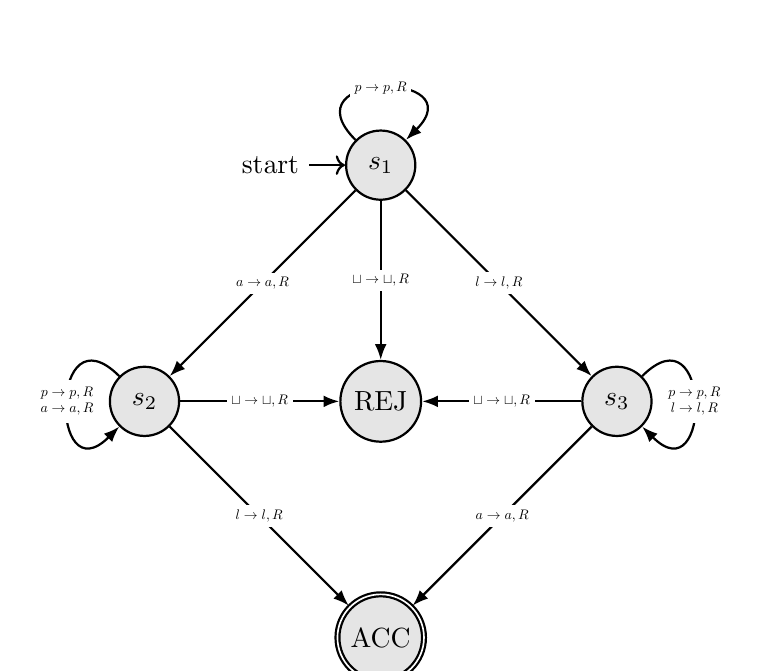
\begin{tikzpicture}
		\node[state, initial] (1) {$s_1$};
		\node[state, below of = 1] (r) {REJ};
		\node[state, left of = r] (2) {$s_2$};
		\node[state, right of = r] (3) {$s_3$};
		\node[state, accepting, below of = r] (a) {ACC};
		\path[-{Latex[length=2mm]}]
			(1) edge [out=135,in=45,looseness=5] node[trans]{$p \rightarrow p,R$} (1)
			(1) edge node[trans]{$a \rightarrow a,R$} (2)
			(1) edge node[trans]{$l \rightarrow l,R$} (3)
			(1) edge node[trans]{$\sqcup \rightarrow \sqcup,R$} (r)

		(2) edge [out=135,in=225,looseness=5] node[trans]{\begin{tabular}{c}$p \rightarrow p,R$\\$a \rightarrow a,R$\end{tabular}} (2)
			(2) edge node[trans]{$l \rightarrow l,R$} (a)
			(2) edge node[trans]{$\sqcup \rightarrow \sqcup,R$} (r)

			(3) edge [out=45,in=315,looseness=5] node[trans]{\begin{tabular}{c}$p \rightarrow p,R$\\$l \rightarrow l,R$\end{tabular}} (3)
			(3) edge node[trans]{$a \rightarrow a,R$} (a)
			(3) edge node[trans]{$\sqcup \rightarrow \sqcup,R$} (r);
	\end{tikzpicture}
\end{figure}

\newpage
\subsection*{Exercise 2}

Let the alphabet $A = \{ 0, 1, 2, 3, 4, 5, 6, 7, 8, 9 \}$. Write
down the algorithm of an enumerator that prints out EXACTLY ONCE
every string in the language $L = \{\ 3m + 1\ |\ m \in \mathbb{N}\ \}$
that is EVEN.

\subsubsection*{Solution}

Note that $L = \{\ 3m + 1\ |\ m \in \mathbb{N}\ \} \text{ that is even} = \{ m \equiv 4 \mod 6\ |\ m \in \mathbb{N}\ \}$.
Let $M$ be a Turing machine that decides language $L$.
The algorithm of $M$ would be as follows:
\begin{enumerate}
	\item
	If the current cell is $4$, move right and go to step 5.
	If the current cell is $\sqcup$ or this is the initial state and the current cell is $0$, REJECT.
	Otherwise, move right and go to step 4.
	\item
	If the current cell is $0$ or $6$, move right and go to step 5.
	If the current cell is $\sqcup$, REJECT.
	Otherwise, move right and go to step 4.
	\item
	If the current cell is $2$ or $8$, move right and go to step 5.
	If the current cell is $\sqcup$, REJECT.
	Otherwise, move right and go to step 4.
	\item
	If the current cell is $0$, $3$, $6$ or $9$, move right and go to step 1.
	If the current cell is $1$, $4$ or $7$, move right and go to step 2.
	If the current cell is $2$, $5$ or $8$, move right and go to step 3.
	Otherwise, REJECT.
	\item
	If the current cell is $0$, $3$, $6$ or $9$, move right and go to step 1.
	If the current cell is $1$, $4$ or $7$, move right and go to step 2.
	If the current cell is $2$, $5$ or $8$, move right and go to step 3.
	Otherwise, ACCEPT.
\end{enumerate}

Note that $M$ always decides if a string of length $n$ characters belongs to $L$ within $n$ steps.
Therefore, it is very easy to print every string in $L$ exactly once by running $M$ on every string in $A^{*}$.
As proven in lectures, $A^{*}$ is countably infinite.
As such, $A^{*}$ is enumerable as a sequence like $A^{*} = \{ w_1, w_2, w_3, \ldots \}$.
Then the enumerator which prints every string in $L$ exactly once =
\begin{enumerate}
	\item Repeat the following for $i = 1,2,3,\ldots$
	\item Run $M$ for $\#{w_i}$ steps on input $w_i$.
	\item Print out $w_i$ if it is accepted.
\end{enumerate}

\subsection*{Exercise 3}

\subsubsection*{Part (a)}

Prove that the emptiness testing problem for phrase structure
grammars (PSG's) given by the language
\[ E_{PSG} = \{\ \langle G \rangle\ |\ \text{G is a phrase structure grammar and}\ L(G) = \emptyset\ \} \]
is Turning-decidable.

\subsubsection*{Solution}

Let there be a Turing machine such as\\
$M$ = on input $\langle G \rangle$
\begin{enumerate}
	\item Mark all terminal symbols in $G$.
	\item Repeat until no new symbol gets marked:
	\item Mark non-terminal $\langle T \rangle$ if $G$ contains a rule $r_1,\ldots,r_i,\langle T \rangle,r_{i+2},\ldots,r_j \rightarrow w_1,\ldots,w_k$ where every symbol except $<T>$ has already been marked.
	\item If the start symbol $\langle S \rangle$ is marked, REJECT. Otherwise, ACCEPT.
\end{enumerate}

The phase structure grammar will generate at least one string if the start symbol $\langle S \rangle$ is markable by the Turing machine $M$.
Therefore, $M$ rejects $G$ if $L(G) \ne \emptyset$ and as such $E_{PSG}$ is Turing-decidable.

\end{document}

